%XXX Since design will focus on each component, this section can mirror the previous chapter, but instead of high level overview, describe how you implemented the description from the design chapter, programming language, libraries etc.

% Python
% Data collection - ccxt, binance, coinmarketcap
% historica data - anomaly detection - matplotlib -ohlcv - pandas - numpy 
% labeling - matplotlib - ohlcv - anomaly d
% generating dataset

\chapter{Implementation of \project}\label{ch:implementation}\glsresetall
This chapter describes the implementation of \project. It first, define which programming language and modules we use during the implementation. Then it details how we implement each component.

We implement the system in the programming language \href{https://www.python.org/}{Python}, which we is a powerful high-level scripting language that is excellent for building prototypes and conducting experiments. It has an extensive and superb standard library, but it also has an active community which provides specialized software that implements various protocols, \acp{api}, etc. It has roots in multiple programming paradigms like procedural, object-oriented, and functional. In recent year, it has climbed to the very top of being the most popular programming language according to PYPL\footnote{Popularity of Programming Languge}~\cite{pypl_python}.

Python has an interpreter, a program that executes the code. Each python interpreter has a \ac{gil}, which is a mutex that protects access to the Python object, preventing multiple threads from executing Python bytecodes at once. This lock is necessary mainly because CPython's memory management is not thread-safe~\cite{python_gil}. Because of the \ac{gil}, a single interpreter cannot execute threads in parallel. To run parallel code in python, we must launch multiple interpreters. If we refer to a process, we refer process with its own interpreter, and we use a thread, then we refer to a thread that's running within an interpreter.

The modules we use are all available from PyPI\footnote{Python Package Index}, a python software repository, and they are all easily installable by using PyPI's package installer pip. The following modules we take advantage of are:

\begin{itemize}
    \item \textbf{ccxt} - package containing a uniform \ac{api} for supporting numerous exchanges.
    \item \textbf{keras} - high-level deep learning network \ac{api}.
    \item \textbf{numpy} - fundamental scientific computing module.
    \item \textbf{pandas} - library containing data structures and data analysis tools.
    \item \textbf{matpotlib} - plotting library.
    \item \textbf{time-series} - module for working with time-series data.  
    \item \textbf{scikit-learn} - tools for data mining and analysis.
    \item \textbf{python-binance} - Python implementation of the exchange Binance.
    \item \textbf{CoinMarketCapAPI} - Python implementation of the cryptocurrency tracking site CoinMarketCap.
\end{itemize}

\section{Data Retriever}
%% MS
% Master
% Slaves - polymorphism
% Dataframe
We implement our data retriever like a master/slave architecture in Python as we described in \autoref{sec:ms}, where the master is a process, but the slaves are threads. The slaves are assigned a source, and they will continuously pull data from the markets as long as they do not exceed their designated source request rate. Then, in a fixed interval, the master collects all the data from the slaves. All the slaves are different types, but they have the same \emph{interface}, allowing the master to exploit the computer science concept \emph{polymorphism} when retrieving the data from the slaves. 

\autoref{code:interface} is the interface for each slave. The initializer method \texttt{\_\_init\_\_} initialize the internal state of each slave, and it gives each slave all the markets it has to fetch data from. The \texttt{start} and \texttt{stop} will make the slave starting and stopping retrieving market data, respectively. The \texttt{header} returns the name of each feature in a market, while \texttt{row}, parses the data then returns the features in the same order as the header. This procedure is done for each market, and the market features will continuously change as the slave fetch new data and updates them.

\begin{lstlisting}[language=python, caption={Slave interface}, label=code:interface]
    class Slave(Thread)
        def __init__(self, markets):
        def header(self):
        def start(self):
        def stop(self):
        def row(self, market):
\end{lstlisting}

The first batch of data the master receives from the slaves, the master augments and stores all the headers (feature description) as the first row in a file, making it similar to a data frame like \autoref{tab:dataframe} illustrates. Where the columns $c$ is the name of each feature, and the rows are enumerated. The data gets parsed such that each feature $f$ gets added to their corresponding column $c$. The succeeding the data batches the master receive gets parsed to a sample and appended to its file. Naming each column is convenient when pulling data from multiple sources as it becomes easy to identify each features in the data, and it will become practical when processing the data. Instead of indexing each feature by number.

\begin{table}[ht]
    \centering
    \begin{tabular}{| r | r r r r |}
        \hline
                    & $c_1$     & $c_2$     & $\dots$   & $c_n$     \\
        \hline
        $1$         & $f_{1,1}$ & $f_{1,2}$ & $\dots$   & $f_{1,n}$ \\
        $2$         & $f_{2,1}$ & $f_{2,2}$ & $\dots$   & $f_{2,n}$ \\
        $\vdots$    & $\vdots$  & $\vdots$  & $\ddots$  & \vdots    \\
        $m$         & $f_{m,1}$ & $f_{m,2}$ & $\dots$   & $f_{m,n}$ \\
        \hline
    \end{tabular}
    \caption[Definition - Dataframe ]{A dataframe can be thought of as a dictionary-like container. Where the columns $c$, are names and represents keys, while the features $f$ are values that are mapped to a column.}
    \label{tab:dataframe}
\end{table}

\subsection{Sources}
We implement three slaves where each slave is asssigned a source. The first slave is pulling data from the exchange Binance by using the module python-binance, the second is pulling data from multiple exchanges with the help of the module ccxt. Finally, the third slave pulls data from the cryptocurrency tracking site CoinMarketCap by using a module we create.

\subsubsection{Binance}
The exchange Binance provides various types of services through their \ac{api}, however, we require only the newest trading data regarding the given markets. We use their \ac{ws} api that takes form as a pubsub client where the Binance push data to us. The first function that we subscribe on is the \emph{ticker} service, a $24$ hour rolling window containing statistics for a subscribed symbol that gets pushed every second~\cite{binance_git}, \autoref{binance_tick} shows the \ac{json} structure of the response of a ticker, and this response is returned for each market we subscribe on. In the ticker response, there are \ac{ohlcv} values for the past 24 hour and other additional features that may prove useful when classifying \ac{pd}.

\begin{lstlisting}[language=json, caption={Ticker response from Binance (Source \cite{binance_git})}, label=code:binance_tick, firstnumber=1]
{
  "e": "24hrTicker",  // Event type
  "E": 123456789,     // Event time
  "s": "BNBBTC",      // Symbol
  "p": "0.0015",      // Price change
  "P": "250.00",      // Price change percent
  "w": "0.0018",      // Weighted average price
  "x": "0.0009",      // First trade(F)-1 price
  "c": "0.0025",      // Last price
  "Q": "10",          // Last quantity
  "b": "0.0024",      // Best bid price
  "B": "10",          // Best bid quantity
  "a": "0.0026",      // Best ask price
  "A": "100",         // Best ask quantity
  "o": "0.0010",      // Open price
  "h": "0.0025",      // High price
  "l": "0.0010",      // Low price
  "v": "10000",       // Base asset volume
  "q": "18",          // Quote asset volume
  "O": 0,             // Statistics open time
  "C": 86400000,      // Statistics close time
  "F": 0,             // First trade ID
  "L": 18150,         // Last trade Id
  "n": 18151          // Total number of trades
}
\end{lstlisting}

Furthermore, we also want the order book from Binance as this may prove useful later. Hence, in addition to subscribe on the ticker symbol we also subscribe on \emph{depth} function from Binance. This function will return a response similar to \autoref{code:binance_depth}.
\begin{lstlisting}[language=json, caption={Depth response from Binance (Source \cite{binance_git})}, label=code:binance_depth, firstnumber=1]
{
  "lastUpdateId": 160,  // Last update ID
  "bids": [             // Bids
    [
      "0.0024",         // Price
      "10"              // Quantity
    ]
  ],
  "asks": [             // Asks
    [
      "0.0026",         // Price
      "100"             // Quantity
    ]
  ]
}
\end{lstlisting}

\subsubsection{ccxt}
The second slave use the ccxt module, which provides a unifrom \ac{api} access to numerous exchanges, and we use module to fetch \ac{ohlc} values from multiple exchanges. In addition, we can also estimate the ratio of how many exchanges that lists a given market. However, there are some complications with using this module because it provides a uniform access to over $100$ exchanges, which becomes troublesome when the slave is initiated with the markets it has to fetch data from.

Thus, we first create a reverse map, where we map markets to a list of exchanges. This is done by initiating all the exchanges from the module and request all the exchanges' markets, and then filtering out the markets who was not initiated with the slave. Then, we create pubsub system that wraps around exchanges, where the system takes a market and a callback function. Now we can effortlessly subscribe to markets in an exchange and with the callback function we seamlessly direct the result, like \autoref{fig:ccxt} illustrated. Also, we to synchronize all the request, each exchange issues the requests simultaneously and stores when all exchanges has gotten a response. 

\begin{figure}
    \centering
    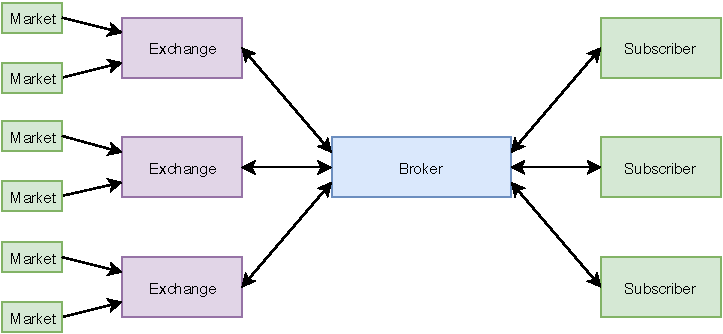
\includegraphics[width=\textwidth]{marketpull.pdf}
    \caption{blablabla}
    \label{fig:ccxt}
\end{figure}

In addition, with the reverse map we create, we can estimate the ratio of how many exchanges that has a given market. As this was one characteristics of a \ac{pd} described in \autoref{tab:pd_characteristics}. Before the master collects the \ac{ohlc} market values, we take the mean of them.

\subsubsection{CoinMarketCap}
The final slave retrieve data from \href{https://coinmarketcap.com/}{CoinMarketCap}, which is a popular cryptocurrency tracking site and contains general information regarding coins like its capitalization, circulation, and etc. We have to use CoinMarketCap private \ac{api} as they deprecated their public \ac{api}. Using their private \ac{api} is relatively intuitive, the identification is an \ac{api} key, but CoinMarketCap has defined a severe complex request system. Where a user has a load of credits, and the amount of credit one have depends on the type of subscription. In addition, a user also has a daily, weekly, and monthly request rate system, which also depends on the type of subscription on have. There are some Python modules in existence that allows one to extract data from CoinMarketCap, but they completely ignore the request system, which, when used will be problematic as we continuously will exceed the request limit and credit system, which ultimately results in a permanent ban from using their \ac{api}.

Thus, we create our own module that support throttling of requests, which adjusts to both the credit system and the number of request one can issue. We cache every request in a database because CoinMarketCap mostly provide data that rarely or slightly change. The cache also comes with an exceed factor allowing one to adjust when cached data shall be removed from the cache. There are four endpoints in CoinMarketCap, where each endpoints has a set of functions:
\begin{itemize}
    \item Cryptocurrency
    \item Exchanges
    \item Globals
    \item Tools
\end{itemize}

We use the modules requests, requests\_cache, and ratelimit. The requests module is module for making requests. Requests\_cache is monkey patch to the request module, and caches every request made by the request module. The ratelimit allows to define function descriptors that restricts the number of function calls within a time scope.

With the module we create, we fetch data from the cryptocurrency endpoints. The majority of the functions in CoinMarketCap requires a paid subscription. We are only using two free functions. The first function returns the global metrics, which contains the important value, total market capitalization. The second function lists cryptocurrencies latest market data that contains the fields circulation supply for each market, it defines the total amount of cryptocurrency worth. The reason we do not use the trading data that CoinMarketCap is because we cache every request, resulting in using stale trading data.

\section{Data Processing}
After gathered enough data, we can start process it. Each market has it own file containing data from all the sources recently described, and since they has to be processed equally, we can parallelize each operation, allowing us to speedup the data processing stage. Each file we have to process can be small in general, but combining them all together they may become quite large. Hence, we only process a fixed number of files in parallel. 

We paralellize every operation by allowing the master process to spawn new child processes. The master initialize every child process with a semaphore and queue. The first process do when they wake up is to grant access to run in a critical space, if their request gets rejected, they has to wait in queue. Once gets inside the critical area, they load the dataset using Pandas and execute the operation they are assigned to do. After they are done with their task, they signalize to the master process using a queue that they are done, and when leaving the critical section, next child process can enter it.

With data loaded into a date frame in Pandas, we index features by their column name, which makes it convinient when we do cleansing and feature engineering. 
% cleanse

The first number of operations involves cleansing the data. We cleanse by removing corrupted files, in some cases, e.g Binance have deleted markets and removed the possibility of extracting trading data from it, which results in corrupt data. We also remove the features that are not needed, e.g, in \autoref{code:bianance_tick}, the constant categorical field \texttt{symbol} are not needed when classifying \ac{pd}. The last cleansing process we do is to interpolate the data. Values involving price and quantity gets linearly interpolated like we describe in \autoref{ch:design}.

The second series of operation we do is to create new features. We calculate the percentage of change like described in \autoref{ch:design} on all the values we interpolated. Then we create new features from using the timestamp that we added along with the data when it was stored. Finally, we create a new feature that describe the imbalance of the order book.

\section{Collecting pump-and-dumps}
When collecting \acp{pd}, we use an anomaly detection algorithm that marks an interval if there was a significant increase of price and volume in that period compared to the previous periods. We do not use the anomaly detection algorithm with the data that was collected in real-time, as this data is not compliant with the algorithm. Instead, we retrieve historical \ac{ohlc} data from Binance that span over the period we gathered data.

The algorithm takes in a window (list) with a fixed number of \ac{ohlcv} values. The window is smaller than the batch of ordered \ac{ohlc} values receieve. So we create a sliding window module which is wraps round a python list. With the sliding window, it becomes is easy initialize a fixed size list, and when adding new element to the list, the last element will be removed. Just like a fixed size \ac{fifo} structure.

\autoref{binance_kline} illustrates an entry in a response from Binance that contains historical klines. With both the klines and a sliding window, we start to contionoussly add \ac{ohlcv} values that span over one hour to the window until it is full, then we iteratively calculate weather the newest added \ac{ohlc} is an anomaly compared to the other \ac{ohlc} values in the window. The fields we use from the data are \texttt{close} and \texttt{high} when calculating the price anomaly, while we only use the field \texttt{volume} when calculating the volume anomaly. The formula we use is described in \autoref{ch:design}

\begin{lstlisting}[language=json, caption={Historical kline response from Binance (Source \cite{binance_git})}, label=code:binance_kline, firstnumber=1]
[
  [
    1499040000000,      // Open time
    "0.01634790",       // Open
    "0.80000000",       // High
    "0.01575800",       // Low
    "0.01577100",       // Close
    "148976.11427815",  // Volume
    1499644799999,      // Close time
    "2434.19055334",    // Quote asset volume
    308,                // Number of trades
    "1756.87402397",    // Taker base volume
    "28.46694368",      // Taker quote volume
  ]
]
\end{lstlisting}

As we have previously mentioned, anomaly detection algorithm tends to have a high occurrences of false-positive compared to true-positive. So we filter them out by plotting finer-grained \ac{ohlc} values from the period that was flagged anomalous from each market. We can plot these \ac{ohlc} values by using the matplotlib module in Python. The chart that seems like a \ac{pd} occured we keep, otherwise we delete that anomaly.

After filtering out the \ac{pd} that seemingly looks like true positives, we can label the the features we created weather that point was collected during a \ac{pd} or not. We use the same parallize processing model, which we used during the feature engineering stage. where each process is iniated with a semaphore and queue, but also the \ac{pd} the periods where a \ac{pd} happened in the data. Then, the child process loads the dataset and idientify the interval where the \ac{pd} occured, and find the points where largest change in price percent happened. From the highest point, we label the points \ac{pd} where the change in percent was positive.

\section{Deep Learning}
After we have generated labeled datasets, we normalize each of them using the min-max method described in \autoref{ch:design}. To find the smallest and biggest value of each feature require us to process trough all of the datasets in order to find the largest sand smallest value in each feature. Then, when we have these value we have to process normalize every row. We use one functions from the scikit-learn package when normalizing the data.

In our implementation, we use the method undersampling when generating a balanced dataset. So, first we have to collect all the positive samples. Then we simply choose random negative sequences from the dataset until the number of negative and positive samples are equal.

we use the deep learning library Keras for our model, the first layer contains active \ac{lstm} cells, and the second layer contains a single perceptron.

Before training a \acp{lstm} network, we need to resphape our input data, which is a matrix, a 2D shape, into 3D shape. A sample now, is a matrix containing batch of row-vectors within a time lag. Then the third dimensions is simply batch of these new samples. After shaping our data, we can finallyu train our model.

